\chapter{\uppercase{Technology Setup}}

A major driving principle of the presented work is that the methodology needs to be scalable. One reason for difficulties in implementing fault detection and diagnostic algorithms and other optimization methods is that there is a significant amount of initial investment necessary. This initial investment can also be cost prohibitive. 

In more complex schemes, it may be necessary to install additional sensors that are typically not available in commercial HVAC systems. Along with the sensor cost there is the cost to tie the sensors into the BAS. The updated logic will need to be coded by a controls vendor, adding more cost. On a large campus, this reprogramming can also take a significant amount of time to complete. 

Another issue is that of risk. There is risk in that if the controls do not function properly and are too complex for the current building operator, the controls cannot be easily removed and set back to default. 

\section{Proposed Setup}

In the proposed setup, the amount of change to the existing BAS is minimal. The control logic remains exactly the same. A small executable script can be installed on the BAS computer that can host code that will send https request to a remote server holding the historical data and the optimization methods. 

Before this process can begin, the sensors will need to be mapped in a way that the server can understand. 

\figref{} \ref{fig:NetworkFlow} shows potential information flow. Over any time period, historical trend data representing the system is stored in a server. This data may come in one large sync or potentially occur daily or sub-daily. Once enough data has been stored on the server, a client BAS computer (potentially one of many) can make an http request that will essentially carry information related to the current time and what equipment the request is for. Each AHU will have a unique identifier that the main web server understands. 

The web server will implement the methods described in this document and will send a response back to the client with the setpoints for the system that will be near-optimal in a steady-state sense, given the expected conditions at the building and individual zones. 

\subsection{Standards for Transmission}

Standards for the format of information transfer are critical for rapid adoption. An Application  Program Interface (API) is the public interface of methods and routines that allow third-party programmers to develop programs from the base building blocks. 

Another important point of consideration is the format of the data actually being transferred. In the software industry, there are several types of data exchange formats, two popular ones being JavaScript Object Notation (JSON) and Extensible Markup Language (XML). 

The advantage of JSON over XML is that requires less characters to describe simple objects. Unlike XML, it does not support explicit schema definition. 



\begin{figure}
\begin{tikzpicture}

\node [anchor=center,draw] (BASComputer) at (0,0) {\includegraphics[width=3cm, height=3cm]{Images/Desktop_computer_clipart_-_Yellow_theme-MPEdits.png}};

\node [anchor=center,draw] (Server) at (7cm, 0) {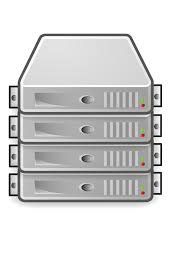
\includegraphics[width=3cm, height=3cm]{Images/serverImage.jpg}};

\draw [->, out=25, in=155, thick,anchor=center ] (BASComputer) to node [yshift=1cm, align=center] {http request \\ \(\approx\)5-15 min} (Server);

\node [above=of Server] {Web Server};

\node [right=of Server, align=left] {Historical data at \\ any syncing interval};

\draw [->, out=225, in=315, thick, ] (Server) to node [yshift=1cm, align=center] {Optimal Setpoints} (BASComputer);



\end{tikzpicture}    
\caption{Diagram of networking flow.}
\label{fig:NetworkFlow}
\end{figure}


\subsection{Advantages to Proposed System}

There are several key advantages to a system similar to the proposed:

\begin{enumerate}
    \item No real-time data transmission. Managing the networking of large BAS systems is difficult enough as is. It is not feasible for a single server to handle live streams of BAS point information from thousands of buildings. 

    \item The system can be added or removed quickly and without side-effects. Because the logic lives at an abstraction level above the BAS code, no changes to the system need to be made locally. 

    \item Routines only have to be added once for different equipment and setup types, allowing the same methods to expand to many different buildings. 


\end{enumerate}
